%---------------------------------------------------------------------------------------------------
% Aufgaben
%---------------------------------------------------------------------------------------------------
\newpage
%\part{Anfang}
\chapter{Aufgaben}
Aufgrund der in der Einarbeitung erworbenen Kenntnisse war es m�glich an folgenden Projekten zu partizipieren. Im Fokus stand die H2-Mobility App, mit einer geringeren Priorit�t folgte die LFI App und zum Schluss gab es noch ein Projekt in dem eine sogenannte Launcher App entwickelt werden sollte. Im folgenden wird auf die verschiedenen Apps eingegangen.

% ----------------------------
\section{H2 Mobility App}
Die App ist f\"ur Besitzer von Wasserstoffautos, also Autos mit einer Brennstoffzelle, gedacht. "Die Brennstoffzelle wird sich durchsetzen"\footnotemark \footnotetext{URL: http://www.spiegel.de/auto/aktuell/wasserstoffauto-die-brennstoffzelle-wird-sich-durchsetzen-a-1235431.html}, ist sich Toyota-Motorenentwickler Gerald Killmann sicher. Daher hat die H2 Mobility Deutschland GmbH \& Co.KG die Firma portrix.net mit der Entwicklung einer App beauftragt die den Nutzern unter anderem das europ�ische Tankstellennetz anzeigt, die Route zur n�chstgelegenen Tankstelle anzeigt, eine Feedback f�r die Tankstellenbetreiber, Schulungsvideos zum Tankvorgang und viele weitere Funktionen bietet.
Die Entwicklung der App erfolgt nach R�cksprache mit dem Vertreter von H2 Mobility und dem f�r das Layout verantwortlichen Designer und wird sowohl f�r iOS als auch f�r Android bei portrix.net programmiert. Features und design-Prototypen werden �ber das digitale Produkt Design Tool InVision an die Programmierer vermittelt und anschlie\ss{}end umgesetzt. Aufgrund der hohen Komplexit\"at und des Umfangs den die App mittlerweile angenommen hat sich das Erscheinungsbild zwischenzeitlich stark ver�ndert. Das organische anwachsen der Funktionalit\"at ist am Versionskontrollbaum gut zu erkennen, da das Projekt beinahe 20000 commits enth�lt.

\subsection{Feedback}
�ber InVision kam die Vorgabe einen Prototyp zu entwickeln, der es erm�glicht einer konkret ausgew�hlten Tankstelle per Knopfdruck ein Feedback zu geben.

\begin{figure}[H]
	\centering 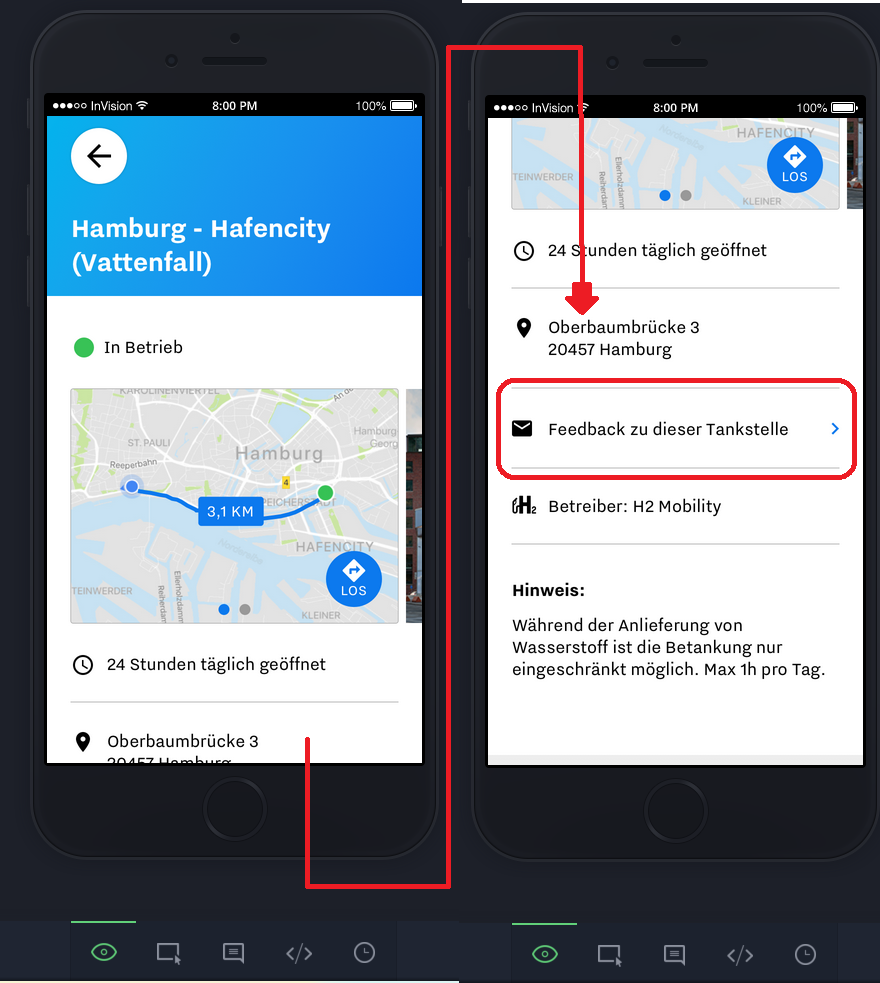
\includegraphics[width=0.8\textwidth]{feedbackPrototyp.png}
	\caption[FeedbackPrototyp]{Prototyp der InVision Vorgabe. Feedback Button f\"ur konkret ausgew\"ahlte Tankstelle}
	\label{fig:FeedbackPrototyp}
\end{figure}
%\footnotetext{URL: https://www.guitarchalk.com/wp-content/uploads/2017/07/electric-guitar-parts.jpg [cited 22 August 2018]}


In der bisherigen Version war es m\"oglich \"uber eine Knopf in der FuelStationsMap.java (MainActivity) das HelpAndFeedback.java (Fragment) aufzurufen und von dort in ein allgemeine Feedback.java (Fragment) zu kommen. Dort l\"asst sich aus einem Spinner, der jede Tankstelle auflistet, eine Tankstelle ausw\"ahlen. Es war also naheliegend den Code zu modifizieren, um aus der FuelStationDetail.java (Activity) direkt in das Feedback.java zu wechseln und die angew\"ahlte Tankstelle direkt im Spinnerfeld anzuzeigen.
Hierzu mussten diverse \"Anderungen vorgenommen werden, da das Feedback.java der darunterliegenden FuelStationsMap.java geh�rt und in der OnCreate() Methode des Feedback.java eine FuelStationsMap Variable als Context initialisiert wird (\ref{code:onCreate}). Dieser Context gew\"ahrleistet unter anderem das der Spinner im Feedback Fragment mit Tankstellen Daten gef\"ullt werden kann. Der Context macht es allerdings unm\"oglich das Feedback.java von einer weiteren Activity, also der FuelStationDetail.java gestartet wird. Es war daher notwendig die FuelStationDetail.java (Activity) als Fragment nachzubauen. 
Der gew\"unschte workflow wird in Abb.(\ref{fig:inVisionFeedbackPrototyp}) dargestellt.

\begin{figure}[H]
	\centering 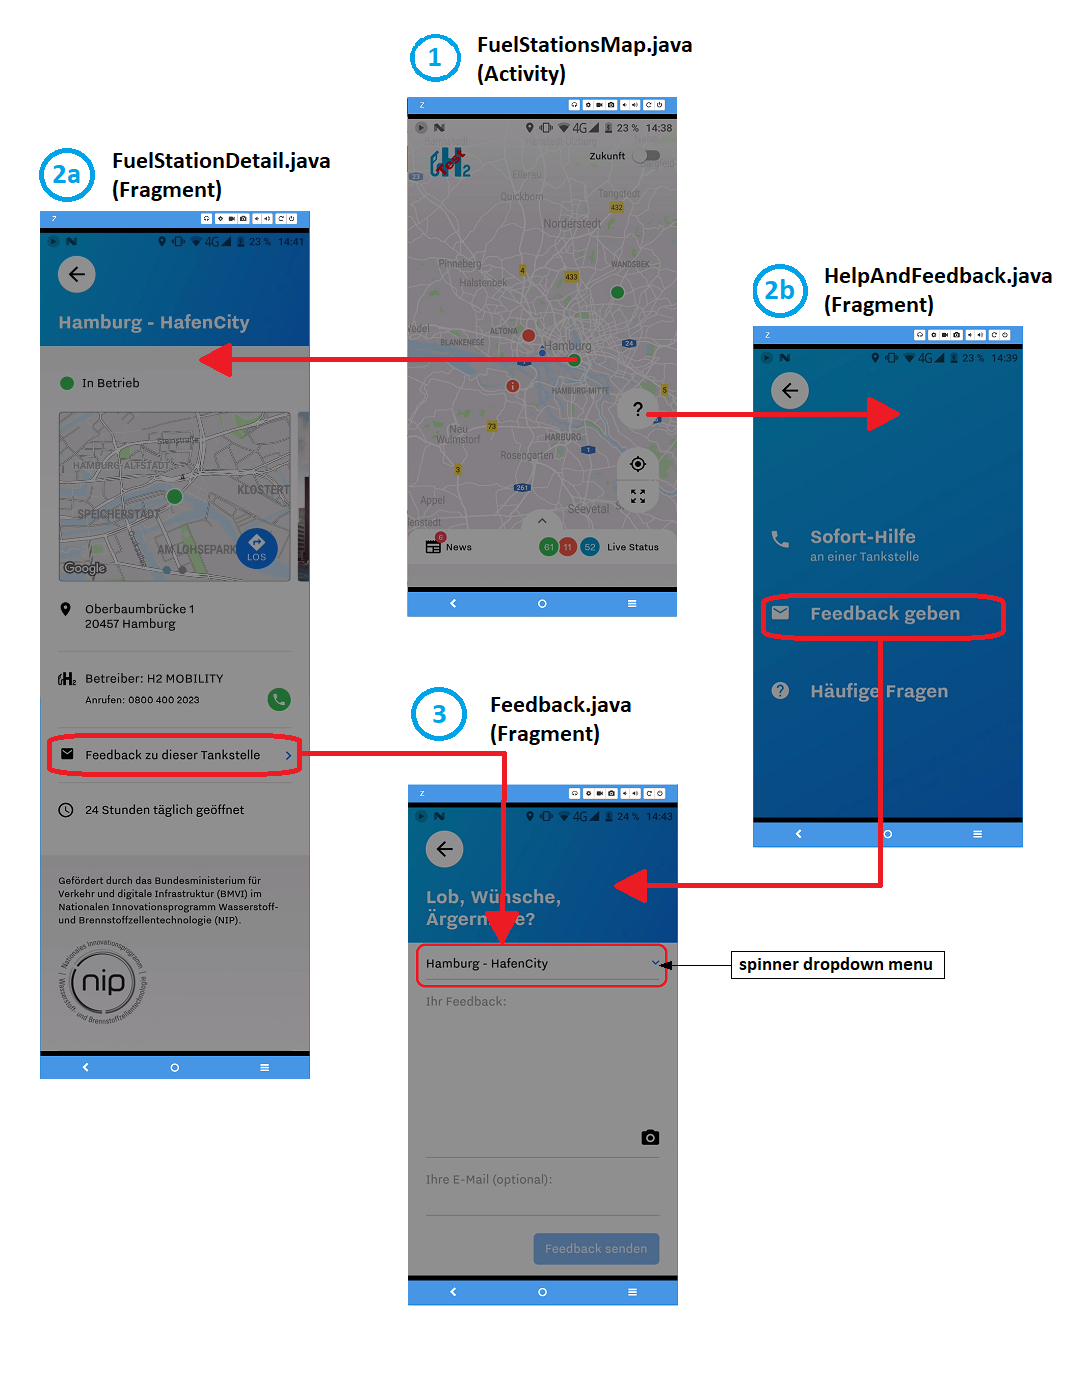
\includegraphics[width=0.8\textwidth]{inVisionFeedbackPrototyp.png}
	\caption[inVisionFeedbackPrototyp]{Workflow der neuen Feedback Funktion}
	\label{fig:inVisionFeedbackPrototyp}
\end{figure}


\fbox{
\lstinputlisting[label={code:onCreate} ,caption={onCreate() Methode der Feedback.java},captionpos=b, language = java]{program/Feedback.java}
}

Das Layout einer App wird in der zur Activity bzw. Fragment zugeh\"origen .xml Datei definiert. In diesem Fall konnte der meiste Inhalt aus der activity\_fuel\_station\_detail.xml in die neue fragment\_fuel\_station\_detail.xml kopiert und um das gew\"unschte neue Feature erg\"anzt werden (\ref{code:feedbackXml}). 

\fbox{
\lstinputlisting[label={code:feedbackXml} ,caption={Designelement Feedback Button},captionpos=b, language = xml]{program/fragment_fuel_station_detail.xml}
}



%--------------
%design vorgabe von Invision
%direktes Feedback im Fragment
%-----------
\subsection{Opt Out}
deaktivieren von Google Analytics

% ----------------------------
\section{LFI App}
super fotografie app
\subsection{Magazin Overview}
neugestaltung der Magazin ansicht
\subsection{Magazin Preview}
Magazin vorschau mit 10 beispielseiten

% ----------------------------
\section{Launcher App}
angesagte Spiegel Tablet